\documentclass[twocolumn,twocolappendix]{aastex631}

\usepackage{amsmath}

\newcommand{\parens}[1]{\left(#1\right)}
\newcommand{\brackets}[1]{\left[#1\right]}

\begin{document}
\author{Jack T. Dinsmore}
\affiliation{Stanford University, Department of Physics}
\title{Inverse Compton Scattering of Accretion Disks in Curved Spacetime}

\begin{abstract}
  Ray-traced images of black hole event horizons, accretion disks, and coronas are presented for the Schwarzschild and Kerr metrics. The physical parameters of the system are adjusted to gain a qualitative understanding of the physics at play in the strongly lensed system.
\end{abstract}

\section{Introduction}

General Relativity (GR) bends the trajectories of light in the presence of strong gravity. Weak examples of this ``gravitational lensing'' present useful techniques in cosmology \citep{blandford1992cosmological}. Near compact objects such as black holes (BH), light is bent so strongly it may curve into a circular orbit or be consumed by the BH's event horizon (EH). Here, computationally intensive methods such as ray-tracing must be employed to model the lensing effect.

Ray-tracing is the act of numerically integrating the equation of motion of a photon along its path to model radiative dynamics \citep{vincent2011gyoto}. The technique is employed in many scenarios. One example is the imaging of accretion disks, which has been simulated as far back as in the 70s \citep{luminet1979image} and observed in 2019 by the Event Horizon Telescope (EHT) \citep{collaboration2019first}. Even when the accretion disk is not resolved, strong lensing is still a crucial effect. Examples include BH spectra \citep{cunningham1975effects}, polarization \citep{dovvciak2008thermal}, and electromagnetic signatures from BH mergers \citep{d2018electromagnetic}.

A benefit of ray-tracing is that it allows the accurate modeling of complicated radiative features of a BH, such as an accretion disk and a corona. An accretion disk is a large disk of cool matter accelerating into the BH, fed by nearby stars or other matter sources, and radiating thermally. The total radiation of this disk is bounded by the Eddington luminosity, above which the radiation pressure produced by accretion would prevent more matter from falling into the BH, thereby lowering the accretion rate back below the Eddington luminosity.

A BH corona consists of matter which has freely fallen from far away into the BH, picking up considerable kinetic energy. This matter collides with other infalling matter and thermally equilibrates, ionizing and becoming very hot. The stripped electrons contain enough thermal energy to be relativistic and can Inverse-Compton (IC) scatter photons from the disk into higher energy bands such as X-rays or $\gamma$-rays.

In this project, we construct a simplified supermassive BH system consisting of a cool accretion disk and a hot corona. Images of the EH and its surroundings are created in the optical band and the X-ray band as various components of the system are modeled. This gives a qualitative understanding of the effect of model components such as strong lensing, accretion disk optical depth, and IC scattering. In section \ref{sec:environment}, we derive the key properties of this simple system and discuss the rendering process in section \ref{sec:rendering}. We present the results in section \ref{sec:results}.

\section{Methods}

Our simplified model for a BH depends only on the BH mass and spin $M$ and $a$, disk absorption coefficient $\alpha$, and the corona scale density $\rho_0$ and $\gamma$ factor. For sufficiently distant sources, the cosmological redshift $z$ is also necessary. Fixing these parameters, we derive the system properties.

\subsection{BH Environment}
\label{sec:environment}
\paragraph{Accretion Disk} The BH itself is assumed to accrete at the Eddington limit, generating luminosity 
\begin{equation}
  L_\text{tot} = \frac{4\pi GMm_pc}{\sigma_T}
\end{equation}
where $m_p$ is the mass of the proton and $\sigma_T$ is the Thomson cross section.
We model this luminosity as emitted near the BH and absorbed and re-emitted as black body radiation by the surrounding gas. This gives the gas flux as a function of radius $r$:
\begin{equation}
  \begin{split}
    F(r) &= \frac{L_\text{tot}}{4\pi r^2} \\&= \parens{1.14\times10^{26}\frac{\text{erg}}{\text{s\ cm}^2}}\parens{\frac{M}{M_\odot}}^{-1}\parens{\frac{r}{r_S}}^{-2}.
  \end{split}
\end{equation}
We interpret $F(r)$ as the flux of the accretion disk outside the innermost stable circular orbit (ISCO) at $r = 3r_S$. However, inside the ISCO the disk falls quickly into the black hole for the Schwarzschild geometry, which we model as a linear decrease in luminosity to zero at the EH. The temperature must obey $F = \sigma T^4$ where $\sigma$ is the Stefan-Boltzmann constant, or
\begin{equation}
    kT(r) =(3.2\ \text{keV})\parens{\frac{M}{M_\odot}}^{-1/4}\parens{\frac{r}{r_S}}^{-1/2}.
    \label{eqn:disk-temp}
\end{equation}
This temperature is redshifted by Doppler boosting, gravitational redshift, and cosmological redshift.

Far enough from the BH, this disk extends above and below the plane due to the reduced BH gravity forcing its collapse. Assuming an ideal gas, the vertical density profile of this structure is Gaussian $\rho(z) = \exp[-z^2/(2H^2)]$, with
\begin{equation}
  H(r) = (3.7 \times 10^{-3} r_S) \parens{\frac{M}{M_\odot}}^{-1/8}\parens{\frac{r}{r_S}}^{5/4}.
\end{equation}
The disk is spatially quite thin; even at $10 r_S$ from the BH, the disk is only a few percent of a Schwarzschild radius thick. For the sake of collisions, we therefore model the disk as two-dimensional, with optical depth
\begin{equation}
  \tau(r) = \frac{\sqrt{2\pi}\alpha H(r)}{\hat{\mathbf z} \cdot \hat{\mathbf v}}.
\end{equation}
for absorption coefficient $\alpha$. Unit vectors $\hat{\mathbf z}$ and $\hat{\mathbf v}$ are the normal vector of the accretion disk and the light velocity respectively. We assume $\alpha$ is constant throughout the disk and independent of wavelength.

We model the rotational velocity of the disk as Keplerian, so that each particle has velocity
\begin{equation}
  \beta(r) = \sqrt{\frac{r_s}{2r}}.
\end{equation}
This will blueshift the disk on once side of the BH and redshift it on the other.

\paragraph{Corona} The corona's formation mechanism implies that each constituent particle is at approximately escape velocity before thermalization, with Lorentz factor $\gamma \approx 1 + (r_S/r)^2/2$. Since $r > r_S$, this is only mildly relativistic. After thermalization, $\gamma_p$ remains mostly unchanged and the electron $\gamma_e$ factor is boosted to $(\gamma_e -1) = (\gamma_p - 1) (m_p / m_e)$, so that both particles have the same kinetic energy. These $\gamma$ factors are assumed to be constant throughout the corona. Appendix \ref{app:corona-density} derives the following density distribution of particles under the assumption of hydrostatic equilibrium:
\begin{equation}
  \begin{split}
  \rho(r) = \rho_0 &\left[1 + \parens{\frac{9}{4(\gamma_p-1)}}\parens{\frac{r_S}{r}}\right.\\
  &+ \left. \frac{1}{2}\parens{\frac{9}{4(\gamma_p-1)}}^2\parens{\frac{r_S}{r}}^2\right],
  \end{split}
\end{equation}
where $\rho_0$ represents some scale density.

The boosted electrons IC scatter accretion-disk photons of energy $\mathcal{O}(\text{keV})$ by equation \ref{eqn:disk-temp} to high-energies with cross section $\sigma_C\approx \sigma_T$, since the photon energy is so low compared to the electron mass energy of 0.5 MeV. This means that the probability of a scatter for a photon ray crossing distance $dr = r_S d\ell$ is
\begin{equation}
  \frac{dp}{d\ell} = \frac{r_S \sigma_T}{m_e} \rho(r) = \parens{2.16 \times 10^8\ \frac{\text{cm}^3}{\text{g}}}\parens{\frac{M}{M_\odot}}\rho(r)
\end{equation}
The process of IC scattering boosts the photon energy by a factor of $\sim\gamma_e^2$. This boosted photon will typically have energy greater than to the rest-mass energy of the electron and $\sigma_C$ will be sharply decreased. For this reason, we assume that each photon is IC-scattered at most once.

IC-scattered photons are ejected roughly parallel to the initial electron velocity in this highly relativistic case, so the angular distribution of IC-scattering is the angular distribution of corona electron velocity. We assume that this distribution is isotropic.



\subsection{Relativistic Ray-Tracing}
\label{sec:rendering}

Since BH physics is set in strongly curved spacetime, all radiative processes must take GR into account. We do this by back-propagating the path each light ray takes from the observer to its source. We perform this propagation with a static metric (either Minkowski, Schwarzschild, or Kerr), which defines the metric tensor $g_{\mu \nu}$ and Christoffel symbols $\Gamma_{\mu\nu}^\lambda$. The metric and symbols are derived in \cite{muller2009catalogue}.

The geodesic equation gives that, for a light ray of velocity $u^\mu$,
\begin{equation}
  \frac{d}{d\lambda}u^\mu = -\Gamma^\mu_{\rho \sigma}u^\rho u^\sigma.
  \label{eqn:accel}
\end{equation}
where $\lambda$ is some parametrization of the light's trajectory, obeying 
\begin{equation}
  \frac{d}{d\lambda}x^\mu = u^\mu.
  \label{eqn:vel}
\end{equation}
Eqs.~\ref{eqn:accel} and \ref{eqn:vel} form a coupled system which are numerically integrated with finite step size $d\lambda$. Because we back-propagate the light, $d\lambda < 0$. 

To reduce numerical inaccuracy, every few iterations, the light velocity is adjusted to ensure it is null:
\begin{equation}
  u^\mu u_\mu = u^\mu u^\nu g_{\mu\nu} = 0.
\end{equation}
It is also key to reduce the step size of $d\lambda$ when near a coordinate singularity, such as an EH or the $\theta=0$ axis in spherical coordinates. Near an EH, light is infinitely redshifted meaning that $x^t \rightarrow -\infty$. This can only be achieved if the derivatives of Eq.~\ref{eqn:accel} blow up, so in practice we stop propagating photons too close to the EH or with $x^t$ too large to avoid numerical error.

The only other gravitational effect we model is redshift. Gravitational redshift for a photon produced while at rest $g_{\mu\nu}$ is $1 + z = \sqrt{g_{tt}}$, assuming that the observer is at infinity where $g_{tt} = 1$. Doppler redshift is also included for matter moving relative to the observer.

When a light ray encounters the accretion disk at radial coordinate $r$, we assume that some fraction $1-e^{-\tau(r)}$ of the light was radiated there. We then propagate the remaining $e^{-\tau(r)}$ until it becomes negligibly small or escapes the system. When an IC event occurs, we scatter the light ray in a uniformly random direction. Due to this random scattering, we must repeat each photon path multiple times avoid small-sample noise. This presents the primary barrier from a computational perspective.


\section{Results}
\label{sec:results}
The BH properties we use are displayed in table \ref{tab:props}. The BH mass was chosen to be that of Messier 87, and the corona $\gamma_p$ was chosen to be the value from class. The other parameters were chosen for the sake of making appealing images. A large redshift was chosen to shift accretion disk temperatures into the visible range, and a large spin was chosen to maximize the difference between the Kerr and Schwarzschild metrics. The absorption coefficient corresponds to an average optical depth of $\tau = 1$ at the innermost stable circular orbit (ISCO), and greater towards the edge of the image.

The observer is placed $10r_s$ away from the BH singularity, slightly above the disk. A single image consists of 150,000 rays of light. For images that also include IC scattering, resampling each pixel requires about 6 million simulated photons per image.

\begin{table}[htbp!]
  \centering
  \begin{tabular}{cc}
    \hline \hline 
    Property  & Value \\ \hline
    Mass ($M$) & $2.4 \times 10^{12} M_\odot$ \\ 
    Absorption coefficient ($\alpha$) & $500/r_S\ (1.7\times 10^{-3}$ cm$^{-1}$) \\ 
    Corona scale density ($\rho_0$) & $5 \times 10^{-26}\ \frac{\text{g}}{\text{cm}^3}$ \\ 
    Proton Lorentz factor ($\gamma_p$) & $1.1$ \\ 
    Spin ($a$) & 0 or 0.8 \\ 
    Cosmological redshift ($z$) & 3.5 \\ 
    \hline \hline
  \end{tabular}
  \caption{BH properties used for this paper. $M$ was set to the mass of Messier 87, and $\gamma_p$ was set to the value given in class. The other parameters are chosen to maximize visibility of the effects at play.}
  \label{tab:props}
\end{table}

\begin{figure}[htbp!]
  \centering
  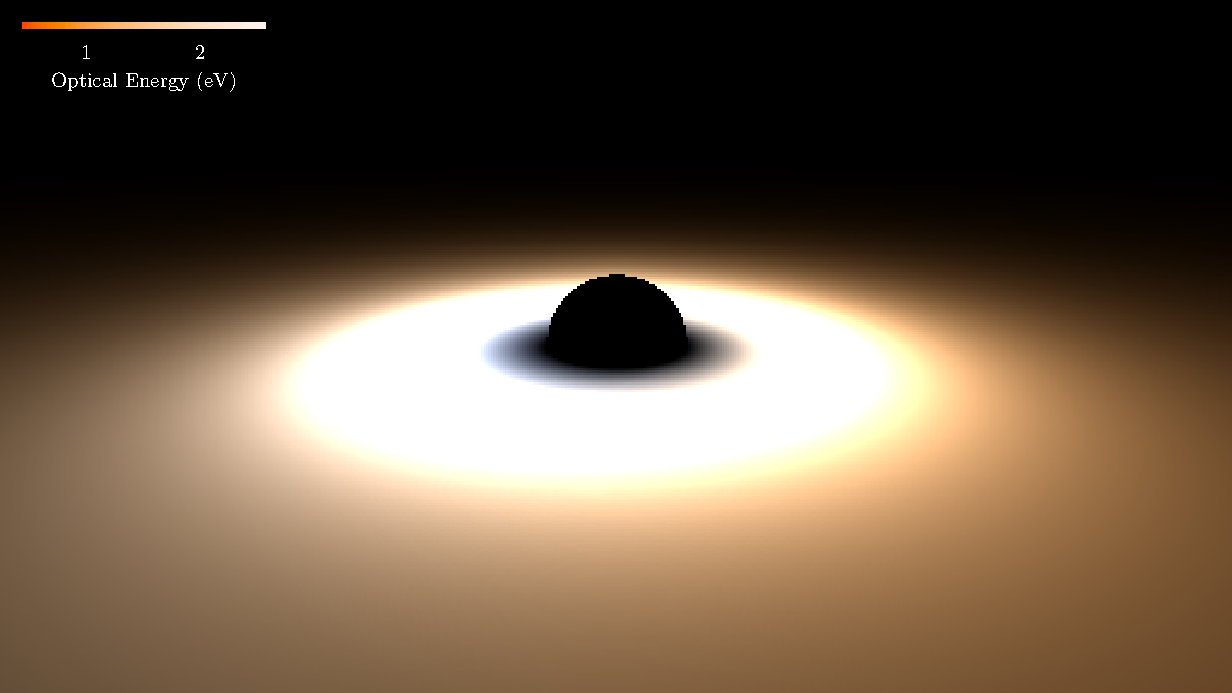
\includegraphics[width=\linewidth]{../imager/small/minkowski-optical.pdf}
  \caption{The accretion disk rendered in Minkowski (flat) space with an opaque ball of the same width as the BH that will be added later.}
  \label{fig:mink}
\end{figure}

Below, each of the BH model components are presented in turn and analyzed in increasing order of complexity. We start with the accretion disk, adding spacetime curvature and studying the effect of accretion depth translucency. Then we consider IC scattering, and finally we consider the Kerr metric. Throughout, the position of the observer will remain fixed. The image brightness is set for each image so that 90\% of the pixels are not saturated, except when otherwise indicated. The color scale shown is the average photon energy $E$, which is related to black body temperature by $E = (hc/bk)kT = 4.97 kT$, where $b$ is Wien's constant.

Figure \ref{fig:mink} displays the accretion disk presented in the flat Minkowski metric. The image shows several key features of the disk, such as its luminosity and temperature dependence on radius and the the Doppler redshift of the accretion disk due to its angular velocity. This Doppler shift is faint, because large $\beta$ only occurs for small $r$, and that region is so bright it appears as mostly white in the image. A black ball with radius $1 r_S$ has been placed in the center with no lensing to depict how small the Schwarzschild radius is compared to the images that will follow. No corona is present in this image.

\begin{figure}
  \centering
  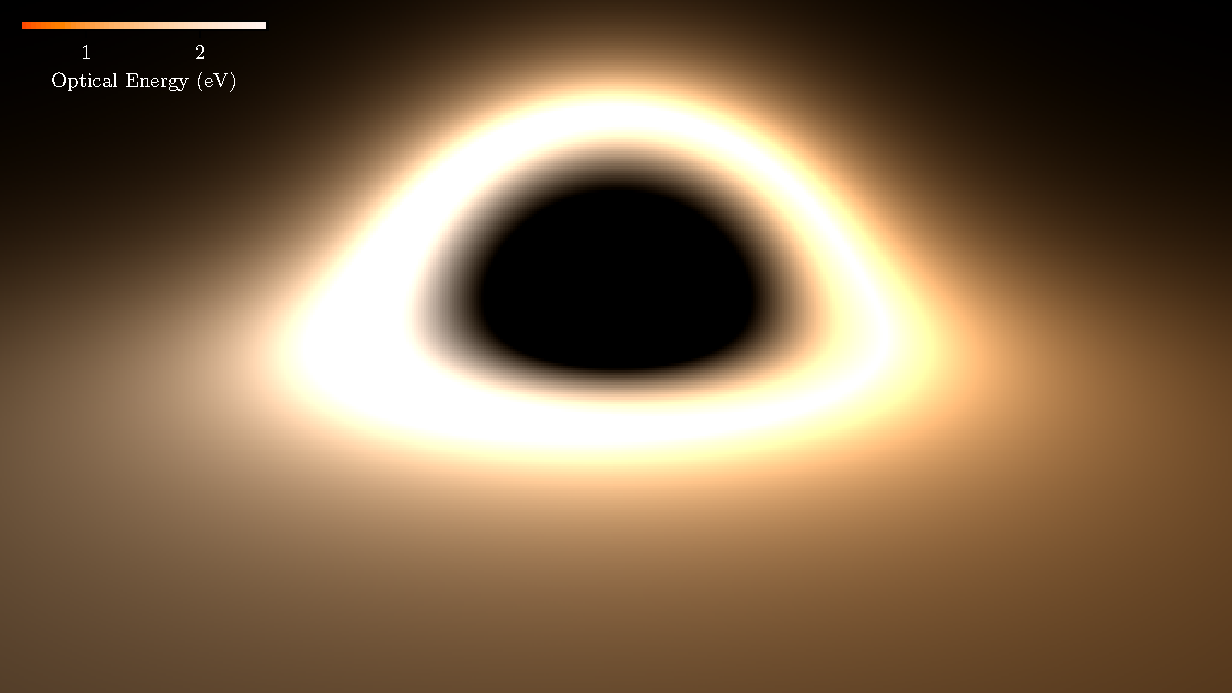
\includegraphics[width=\linewidth]{../imager/small/thick-optical.pdf}
  \caption{The Schwarzschild spacetime with an optically thick ($\tau \gg 1)$ accretion disk. The back of the disk is lensed over the BH and appears higher in the image.}
  \label{fig:thick}
\end{figure}

\begin{figure}[htbp!]
  \centering
  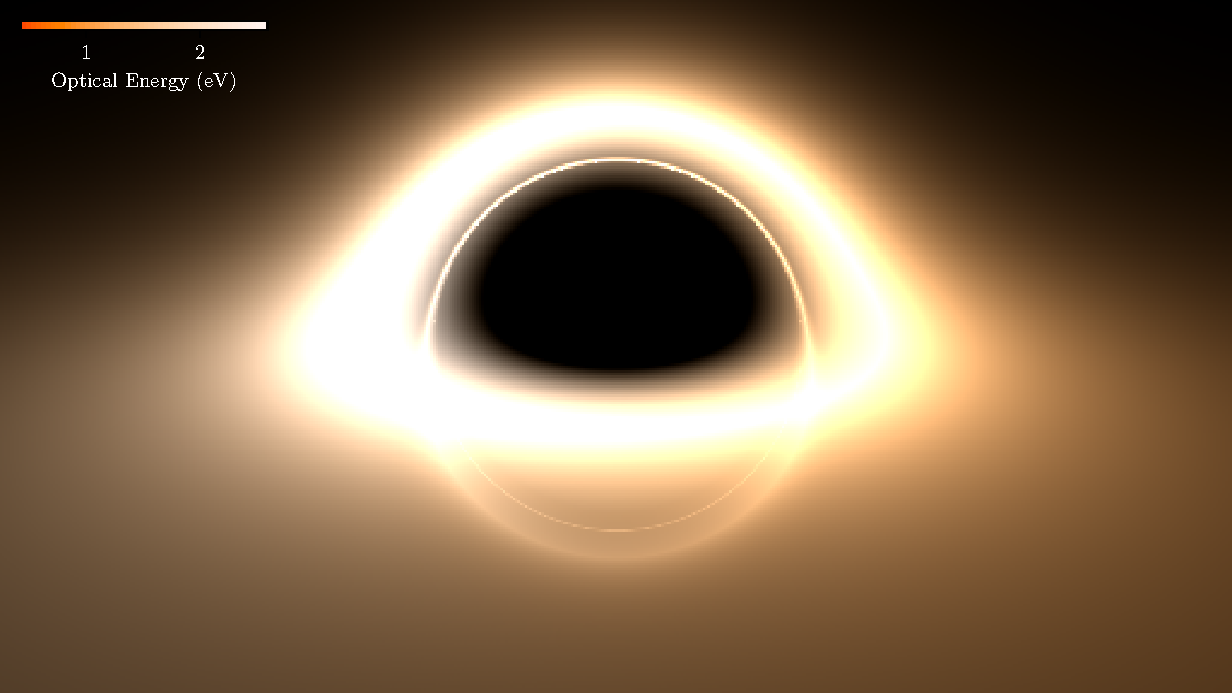
\includegraphics[width=\linewidth]{../imager/small/thin-optical.pdf}
  \caption{(\textit{Top}) The Schwarzschild spacetime with a thinner ($\tau \gtrsim 1$) accretion disk. The BH is observable underneath the disk, and the area around the BH is brighter. The photon ring is also visible as a perfect circle around the BH.}
  \label{fig:thin}
\end{figure}

Figure \ref{fig:thick} shows the Schwarzschild metric added onto the accretion disk depicted in figure \ref{fig:mink}. The absorption coefficient of the disk has been raised to $\tau \gg 1$ throughout the disk, and there is still no corona so that the effect of gravitational lensing is more readily seen. The disk appears to rise above the BH where the BH is lensing light down towards the disk. This part of the disk is therefore more apparent than it was without lensing and, would have a larger effect on general observational properties of the BH, e.g. polarization or spectrum.

Figure \ref{fig:thin} shows the BH system with an accretion disk of the listed $\alpha$. Since some photons are allowed to pass through the disk, the EH is visible below the disk as well as above it. Just outside the bottom EH is a thin halo where light has been bent around the BH and intersects the accretion disk on the other side. This light has impacted the accretion disk twice and therefore contains additional flux, though the far side of the disk is masked by a factor of $e^{-\tau}$. If $\tau$ were lowered, this lower half of the halo would grow brighter rapidly until it overwhelmed the upper half.

Interestingly, the upper and lower halves of the halo display the same parts of the disk. If a transient event occurred in that region, the effect would be visible in flux from the BH at slightly offset times, due to the longer travel time of the lower-half of the halo and the time it takes to pass through the disk. This can affect the light curve of the event, even if the EH cannot be resolved.

Also present in figure \ref{fig:thin} is the photon ring, which is faintly visible as a thin, bright circle just outside the EH. Despite its thinness, the top of the ring is close to brightest part of the image by flux, because it represents light which has gone into nearly circular orbit around the BH and has impacted the accretion disk many times, picking up additional luminosity. Observational evidence for this feature is tenuous, but it is a target for such campaigns as the EHT.

\begin{figure}
  \centering
  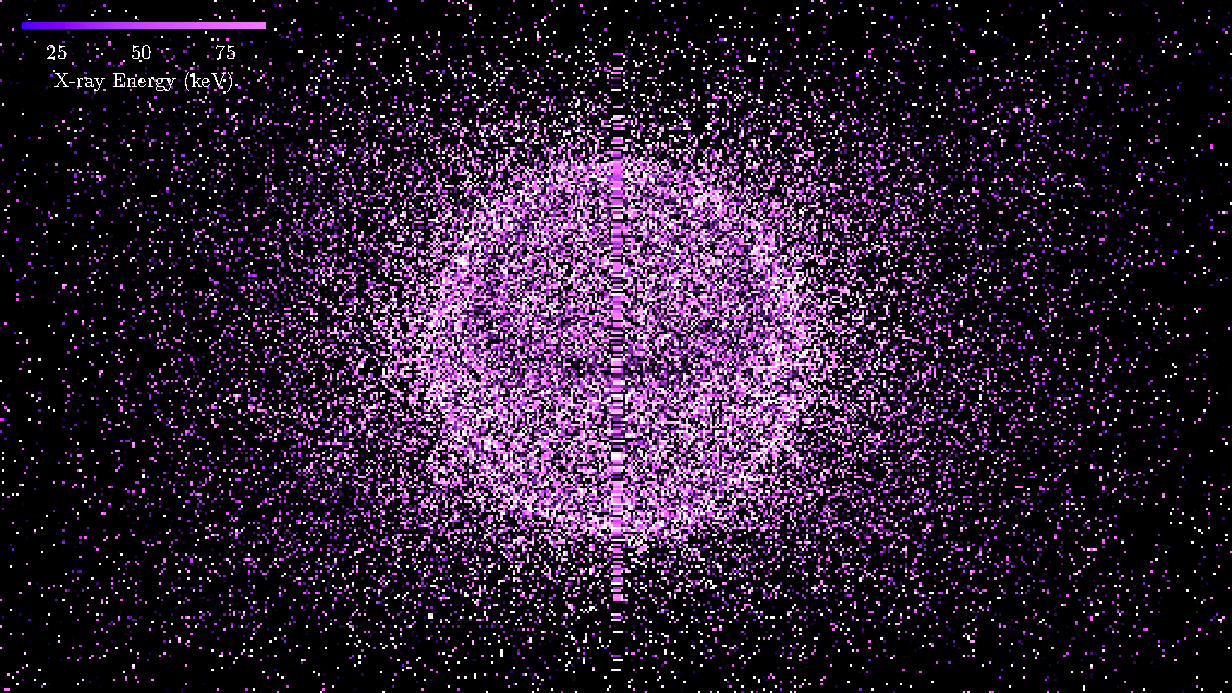
\includegraphics[width=\linewidth]{../imager/small/schwarzschild-xray.pdf}
  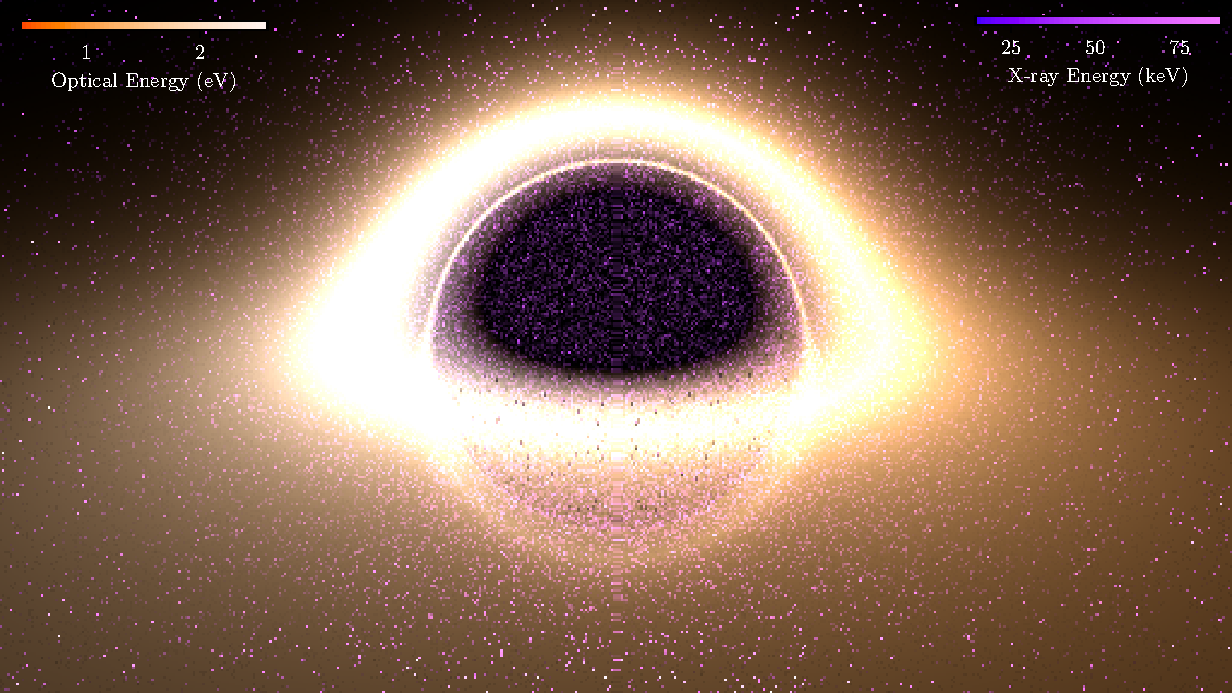
\includegraphics[width=\linewidth]{../imager/small/schwarzschild-tog.pdf}
  \caption{(\textit{Top}) The Schwarzschild geometry in the X-ray band, which contains only IC scattered light. Near-horizon emission is much stronger than in the visible case. (\textit{Bottom}) A composite image showing both X-ray and visible light.}
  \label{fig:sch}
\end{figure}


\begin{figure}
  \centering
  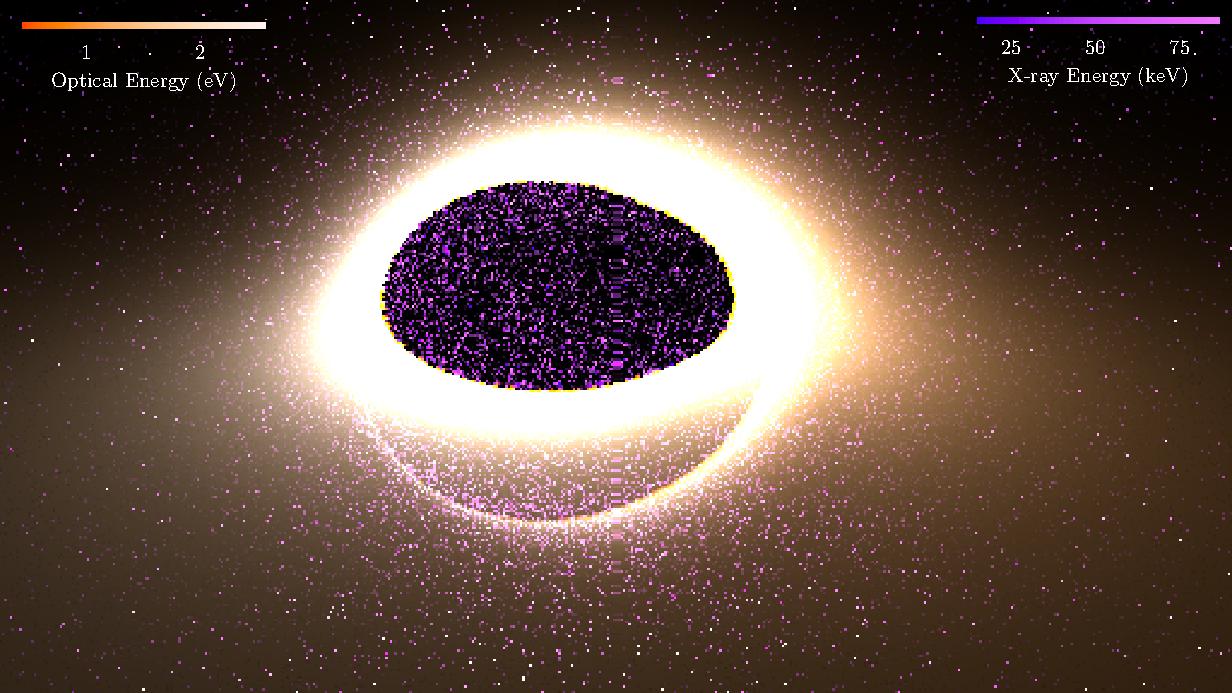
\includegraphics[width=\linewidth]{../imager/small/kerr-tog.pdf}
  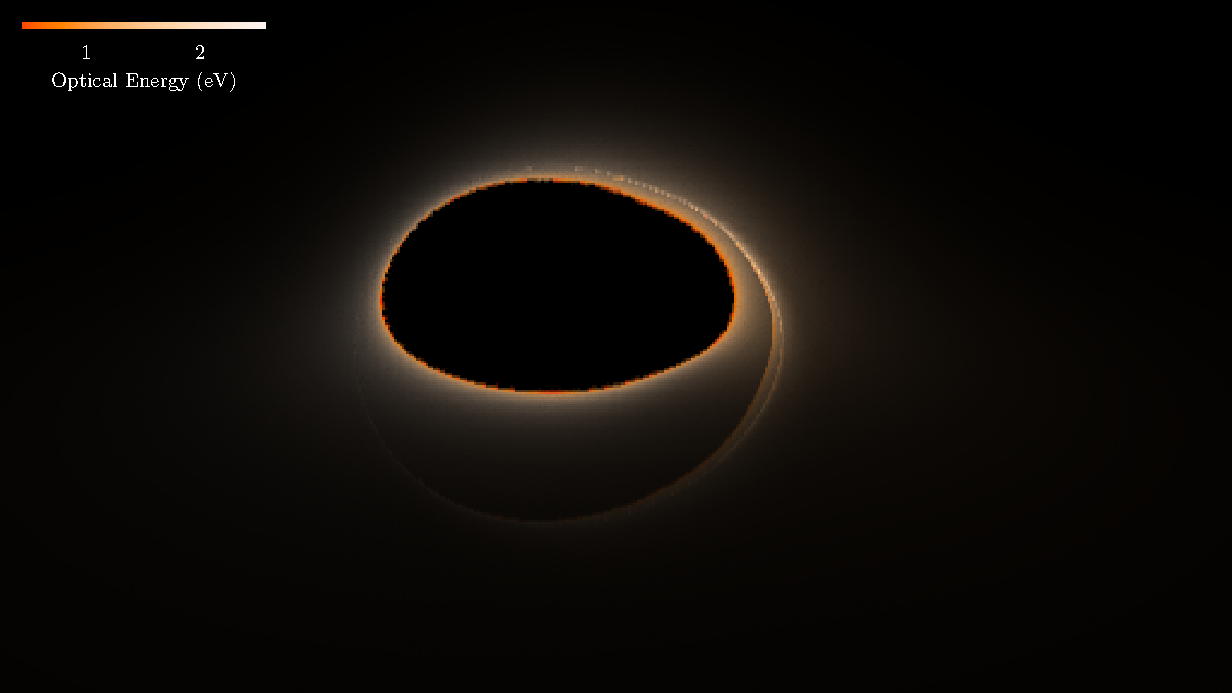
\includegraphics[width=\linewidth]{../imager/small/kerr-bright-optical.pdf}
  \caption{(\textit{Top}) Visible and X-ray emission in the Kerr geometry with $a = 0.8$. (\textit{Bottom}) The brightest pixels in the optical band, exhibiting redshift.}
  \label{fig:kerr}
\end{figure}

Figure \ref{fig:sch} models the corona and depicts the corresponding X-ray flux. By assumption that the corona density $\rho_0$ is small enough that IC scattering is unlikely, the visible flux of the BH is mostly unchanged. The top panel of the figure however depicts an appreciable population of X-rays emanating from all points near the BH, even from regions where visible light cannot emanate. This is due to the ability of IC scattering to change the photon direction. The general distribution of IC photons conforms to the density distribution of the corona, brighter towards the EH. But near the photon ring the IC photon flux is additionally boosted due to the strong likelihood to find photons orbiting the BH in this region, and the brightness of the inner disk. The ring itself is slightly visible, though not as clearly as in the visible case (partly due to the small-count noise of the IC photons). Darker spots representing gravitational redshift are also faintly visible near the very edge of the accretion disk, though the effect is small.

The bottom panel of figure \ref{fig:sch} presents the X-ray counts overlayed on the visible light observed from the BH. This image further highlights the fact that some regions of the image emit only in the X-ray, including the EH above and below from the disk and the space above the accretion disk. This may be interesting from an observational perspective because it means that the properties of the emission are sensitive to different regions of the system depending on their wavelength.
    
We end the discussion of this simple model by presenting the full system for the Kerr spacetime in figure \ref{fig:kerr}. In the Kerr spacetime, we allow the accretion disk to extend all the way down to the event horizon, which contributes more photons to the high-flux, high-corona-density environment near the EH. This increases the X-ray flux due to Compton scattering and allows gravitational redshift to be seen in the optical band much more clearly than the previous examples (bottom panel). The horizon itself has stretched towards the blue-shifted part of the disk, disrupting the photon ring.

\section{Conclusion}

A simple physical model of the environment around a supermassive BH was developed and images of the lensed accretion disk generated for an M87-like system, both in the visible and X-ray bands. Several key qualitative features were observed, such as the amplification of the accretion disk behind the BH due to lensing, the importance of optical depth in the visibility of the lower half of the BH and the photon ring, the small effect of gravitational redshift, the differences in optical and X-ray spatial-distribution, and the effect of BH spin on these phenomena. Ray-tracing models more advanced than this one can be further used to generate quantitative predictions for observables of a specific source, or as a forward model to interpret observations of a BH accretion disk.

\section*{Appendix: Corona density distribution}
\label{app:corona-density}
Assuming Newtonian gravity, the differential force due to pressure on a chunk of matter with volume $dV = r^2 d\Omega dr$ and mass $\rho dV$ is $dP r^2 d\Omega$, and the force due to gravity is $-GM\rho dV / r^2$. The ideal gas law provides $P = \frac{\rho}{m_p}kT$, where we use the proton mass because electrons are comparatively so small. Equilibrium therefore requires
\begin{equation}
  \frac{d\rho}{dr} = -\frac{GM\rho}{r^2}\frac{m_p}{kT}
\end{equation}
assuming that temperature is constant throughout the cloud. The solution is
\begin{equation}
  \rho(r) = \rho_0 \exp \brackets{\frac{GMm_p}{kT}\parens{\frac{1}{r}-\text{const}}}.
  \label{eqn:intermediate-density}
\end{equation}
The kinetic energy per protons is $(\gamma_p-1) m_p c^2$ but also $\frac{9}{2}kT$ by equipartition arguments, since the non-relativistic proton has energy $\frac{3}{2}kT$ and the relativistic electron has energy $3kT$. Since $r_S = 2GM/c^2$, equation \ref{eqn:intermediate-density} can be written as (rescaling $\rho_0$)
\begin{equation}
  \rho(r) = \rho_0 \exp \parens{\frac{9r_s}{4(\gamma_p-1) r}}.
  \label{eqn:density-distro-full}
\end{equation}

This equation becomes extremely large near $r_s \approx r$, but in this region, relativistic effects dominate, making this derivation invalid. Specifically, gravity would dominate over pressure and consume matter near the EH. Taking this effect to the extreme, a corona with no pressure near the EH would show density distribution $\rho(r) \propto \frac{1}{r^2}$ for a constant flow of matter into the BH.

To approximately wed the distant behavior of equation \ref{eqn:density-distro-full} to the near-BH $1/r^2$ in-fall, we Taylor expand the exponential of equation \ref{eqn:density-distro-full} and remove the terms of order $1/r^n$ for $n\geq 3$. This yields the density distribution given in the main text.

\bibliography{bib}{}
\bibliographystyle{aasjournal}



% If the BH consumes corona matter at small $r$, other sources must supply electrons from large $r$ and the entire corona move radially inwards to transport the electrons. Conserving the mass in each region of space requires that this velocity $\beta(r)$ satisfy
% \begin{equation}
%   (d\Omega (r+dr)^2 dr)(\rho(r)+d\rho)(\beta(r) + d\beta) = d\Omega r^2 dr \beta(r),
% \end{equation}
% which corresponds to the differential equation
% \begin{equation}
%   r\rho(r)\frac{d\beta}{dr} +  r\frac{d\rho}{dr}\beta(r) +  2\rho(r)\beta(r) = 0.
% \end{equation}
% Solving this differential equation with $\beta=c$ at $r=r_s$, we get
% \begin{equation}
%   \beta(r) = e^{1/\gamma}\parens{\frac{r_S}{r}}^2\parens{\frac{\rho_0}{\rho}},
% \end{equation}


\end{document}